\chapter{インストール方法}

\section{Node.jsのインストール}

\tacsim のビルドにはNode.js環境が必要になるため, まずはNode.jsのインストールを行う.
\url{https://nodejs.org/ja/}に移動してインストーラをダウンロードし実行することでインストールできる. 正しく実行できたかどうかを確認するためには, 以下のコマンドを実行する.

\begin{mylist}
\begin{verbatim}
$ node --version
v16.15.0
\end{verbatim}
\end{mylist}

\section{\tacsim のインストール}

\tacsim のソースコードは\url{https://github.com/TacSimTeam/TacSimulator-TS}から入手できる. ダウンロードした配布物を展開し以下の順にインストールを行う.

\subsection{依存パッケージのダウンロード}

TacSimulator-TSディレクトリに移動し以下のコマンドを実行する.

\begin{mylist}
\begin{verbatim}
$ npm ci
\end{verbatim}
\end{mylist}

以上で\tacsim のビルドに必要なパッケージを全てインストールできる.

\subsection{\tacsim のコンパイル}

以下のコマンドを実行するとソースコードがコンパイルされる.

\begin{mylist}
\begin{verbatim}
$ npm run compile
\end{verbatim}
\end{mylist}

\section{\tacsim の実行}

TacSimulator-TSディレクトリで以下のコマンドを実行すると, \tacsim が起動する.

\begin{mylist}
\begin{verbatim}
$ npm start
\end{verbatim}
\end{mylist}

成功すると, 画面に\tacsim のウィンドウが表示される.

\begin{figure}[H]
    \centering
    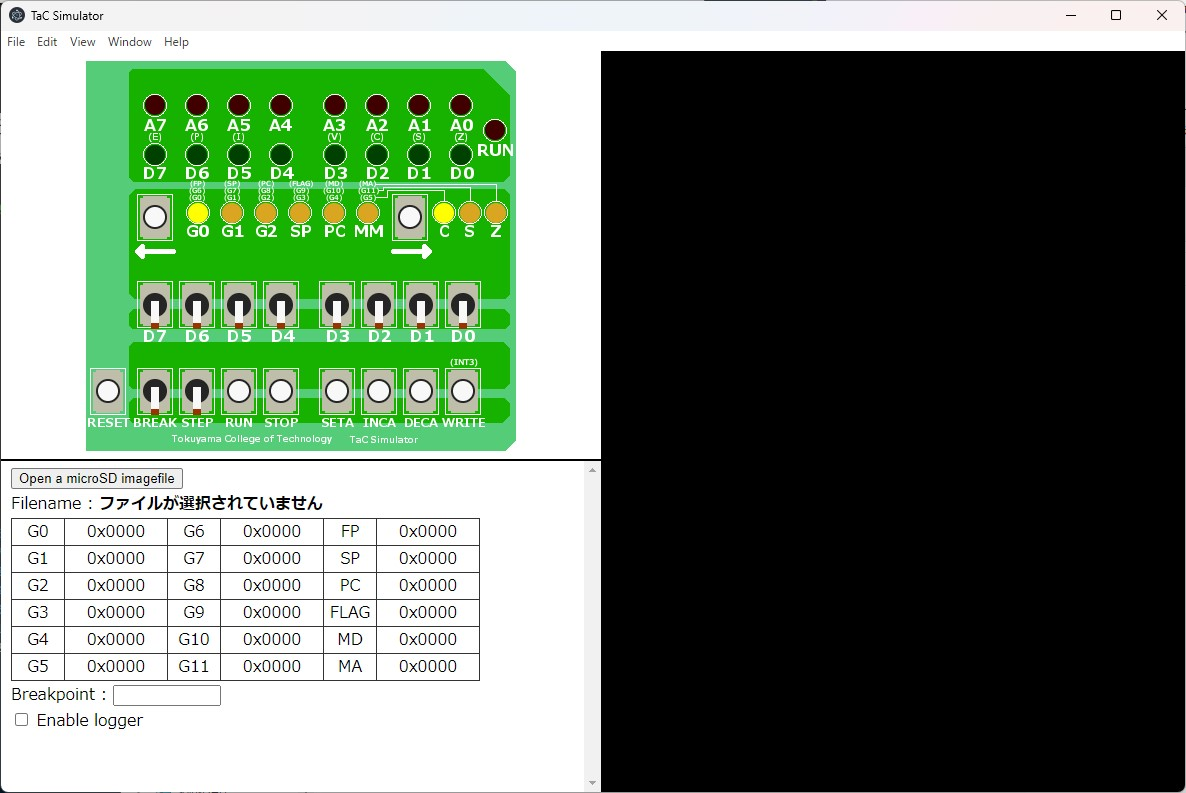
\includegraphics[width=10cm]{"figs/chapter2-tacsimulator.jpg"}
    \caption{\tacsim の画面} \label{fig:ch2-tacsim}
\end{figure}

\section{\tacsim の実行バイナリ作成}

\subsection{Windowsの場合}

以下のコマンドを実行することで, \tacsim のインストーラを生成することができる.

\begin{mylist}
\begin{verbatim}
> npm run build:win
\end{verbatim}
\end{mylist}

成功すると, TacSimulator-TS/TacSimulatorにTacSimulator Setup X.X.X.exeというファイルが生成され, 実行すると\tacsim のインストーラが実行される.

PCにインストールしたくない場合は, TacSimulator-TS/TacSimulator/win-unpackedに実行バイナリが生成されているので, これを実行することでシミュレータを起動できる.

\subsection{macOSの場合}

以下のコマンドを実行することで, \tacsim のインストーラが入ったdmgファイルを生成することができる.

\begin{mylist}
\begin{verbatim}
> npm run build:mac
\end{verbatim}
\end{mylist}

成功すると, TacSimulator-TS/TacSimulatorにTacSimulator Setup X.X.X.dmgというイメージファイルが生成される. 中にはインストーラが入っており, 実行するとインストールが開始される.

PCにインストールしたくない場合は, TacSimulator-TS/TacSimulator/macに実行バイナリが生成されているので, これを実行することでシミュレータを起動できる.
